\begin{figure}
	\centering
	\begin{tabular}{@{}cc@{}c@{}c@{}c@{}c@{}}
		& RGB & Depth & FORTH & Classification & 3-D Pose \\  
		\raisebox{1cm}{\parbox{2cm}{(a) Seq. B frame 303}} & 
		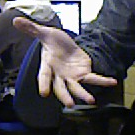
\includegraphics[width=2.4cm]{fig/hand/qual/rgb/image_0303.png} &
		
\includegraphics[width=2.4cm]{fig/hand/qual/depth/image_0303.png} &
		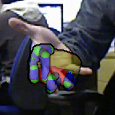
\includegraphics[width=2.4cm]{fig/hand/qual/forth/image_0303.png} &
		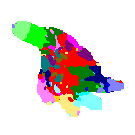
\includegraphics[width=2.4cm]{fig/hand/qual/class/class-303.png} &
		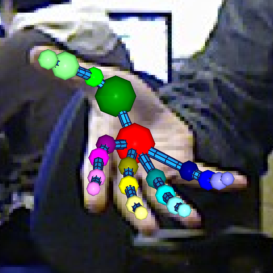
\includegraphics[width=2.4cm]{fig/hand/qual/vote/image_0303.png}
		\phantomsubcaption\label{fig/hand/multi1} \\
		\raisebox{1cm}{\parbox{2cm}{(b) Seq. B frame 520}} & 
		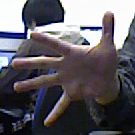
\includegraphics[width=2.4cm]{fig/hand/qual/rgb/image_0520.png} &
		
\includegraphics[width=2.4cm]{fig/hand/qual/depth/image_0520.png} &
		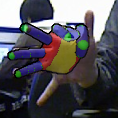
\includegraphics[width=2.4cm]{fig/hand/qual/forth/image_0520.png} &
		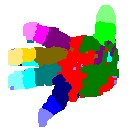
\includegraphics[width=2.4cm]{fig/hand/qual/class/class-520.png} &
		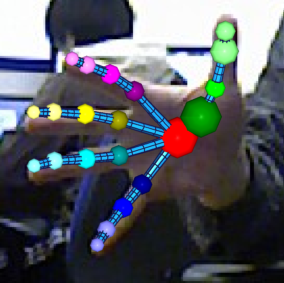
\includegraphics[width=2.4cm]{fig/hand/qual/vote/image_0520.png}
		\phantomsubcaption\label{fig/hand/multi2} \\
		\raisebox{1cm}{\parbox{2cm}{(c) Seq. B frame 825}} & 
		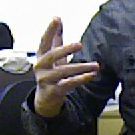
\includegraphics[width=2.4cm]{fig/hand/qual/rgb/image_0825.png} &
		
\includegraphics[width=2.4cm]{fig/hand/qual/depth/image_0825.png} &
		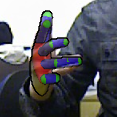
\includegraphics[width=2.4cm]{fig/hand/qual/forth/image_0825.png} &
		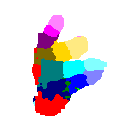
\includegraphics[width=2.4cm]{fig/hand/qual/class/class-825.png} &
		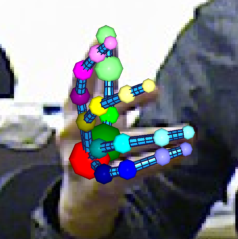
\includegraphics[width=2.4cm]{fig/hand/qual/vote/image_0825.png}
		\phantomsubcaption\label{fig/hand/multi3} \\
		\raisebox{1cm}{\parbox{2cm}{(d) Seq. B frame 946}} & 
		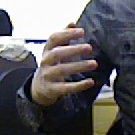
\includegraphics[width=2.4cm]{fig/hand/qual/rgb/image_0946.png} &
		
\includegraphics[width=2.4cm]{fig/hand/qual/depth/image_0946.png} &
		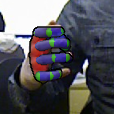
\includegraphics[width=2.4cm]{fig/hand/qual/forth/image_0946.png} &
		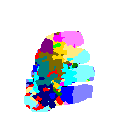
\includegraphics[width=2.4cm]{fig/hand/qual/class/class-946.png} &
		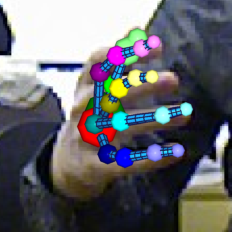
\includegraphics[width=2.4cm]{fig/hand/qual/vote/image_0946.png}
		\phantomsubcaption\label{fig/hand/multi4} \\
		\raisebox{1cm}{\parbox{2cm}{(e) Seq. B frame 996}} & 
		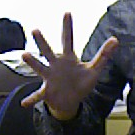
\includegraphics[width=2.4cm]{fig/hand/qual/rgb/image_0996.png} &
		
\includegraphics[width=2.4cm]{fig/hand/qual/depth/image_0996.png} &
		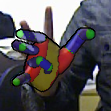
\includegraphics[width=2.4cm]{fig/hand/qual/forth/image_0996.png} &
		
\includegraphics[width=2.4cm]{fig/hand/qual/class/class-996.png} &
		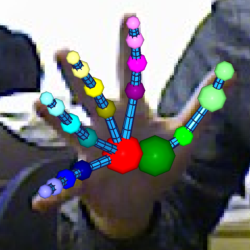
\includegraphics[width=2.4cm]{fig/hand/qual/vote/image_0996.png}
		\phantomsubcaption\label{fig/hand/multi5} \\ 
		\raisebox{1cm}{\parbox{2cm}{(f) Seq. C frame 198}} &
		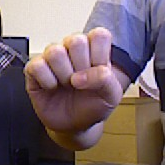
\includegraphics[width=2.4cm]{fig/hand/qual/rgb/image_0198.png} &
		
\includegraphics[width=2.4cm]{fig/hand/qual/depth/image_0198.png} &
		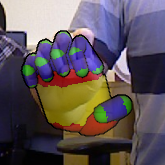
\includegraphics[width=2.4cm]{fig/hand/qual/forth/image_0198.png} &
		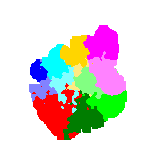
\includegraphics[width=2.4cm]{fig/hand/qual/class/class-198.png} &
		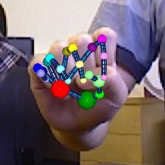
\includegraphics[width=2.4cm]{fig/hand/qual/vote/image_0198.png} 
		\phantomsubcaption\label{fig/hand/multi6} \\
		\raisebox{1cm}{\parbox{2cm}{(g) Seq. C frame 440}} & 
		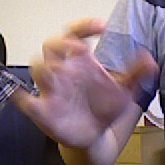
\includegraphics[width=2.4cm]{fig/hand/qual/rgb/image_0440.png} &
		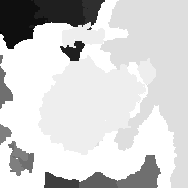
\includegraphics[width=2.4cm]{fig/hand/qual/depth/image_0440.png} &
		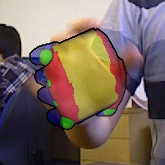
\includegraphics[width=2.4cm]{fig/hand/qual/forth/image_0440.png} &
		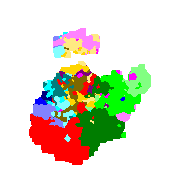
\includegraphics[width=2.4cm]{fig/hand/qual/class/class-440.png} &
		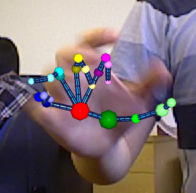
\includegraphics[width=2.4cm]{fig/hand/qual/vote/image_0440.png} 
		\phantomsubcaption\label{fig/hand/multi7} \\
	\end{tabular}
	\caption{Qualitative results of the multi-view experiment. Hand regions are cropped from the original images for better visualisation ($135\times135$ pixels for sequence $B$, $165\times165$ pixels for sequence $C$); the size of the origin images (RGB and depth) is $640\times480$ pixels.}
	\label{fig/hand/multiqual}
\end{figure} 
